\setcounter{ex}{0}% Reset lại số đếm câu hỏi
\Opensolutionfile{ans}[ans/ans-TT-09]
%%==========Câu 1
\begin{ex}%[2D1Y1-2]
	Cho hàm số $f(x)$ có bảng xét dấu đạo hàm dưới đây. Mệnh đề nào sau đây là \textbf{sai}?
	\begin{center}
	
\begin{tikzpicture}
	\tkzTabInit[nocadre=false,lgt=1.2,espcl=2.5]
	{$x$ /1, $y'$ /1}
	{$-\infty$,0,$1$,$+\infty$}
	\tkzTabLine{ ,-,d,-,$0$,$+$ }
	\end{tikzpicture}
	\end{center}
	\choice
	{Hàm số đã cho nghịch biến trên khoảng $(-\infty; 0)$}
	{Hàm số đã cho nghịch biến trên khoảng $(0; 1)$}
	{\True Hàm số đã cho đồng biến trên khoảng $(0;+\infty)$}
	{Hàm số đã cho đồng biến trên khoảng $(1;+\infty)$}
	\loigiai{
	Từ bảng xét dấu đạo hàm ta thấy hàm số nghịch biến trên khoảng $(-\infty;0)$ và $(0; 1)$; đồng biến trên khoảng $(1;+\infty)$. Vậy kết luận hàm số đã cho đồng biến trên khoảng $(0;+\infty)$ là sai.}
\end{ex}
%%==========Câu 2
\begin{ex}%[2D1B5-1]
	\immini{
	Đường cong ở hình bên là đồ thị của hàm số nào sau đây?
	\choice
	{\True $y=x^3-2x^2+3$}
	{$y=-x^3+2x^2+3$}
	{$y=x^4-3x^2+3$}
	{$y=-x^3-2x^2+3$}
	}
	{
	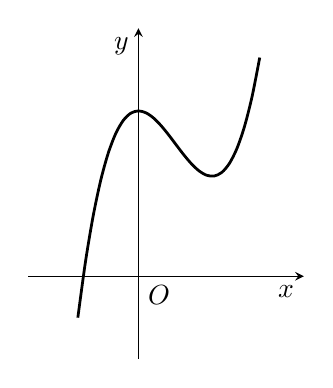
\begin{tikzpicture}[>=stealth,scale=0.7]
	\draw[->] (-2,0)--(0,0) node[below right]{$O$} -- (3,0)	node[below left]{$x$};
	\draw[->] (0,-1.5)--(0,4.5)	node[below left]{$y$};
	\draw[smooth, line width=1] plot[domain=-1.1:2.2] (\x,{(\x)^3-2*(\x)^2+3});
	\end{tikzpicture}
	}
	\loigiai{
	Đồ thị hàm số có hình dạng của hàm bậc ba nên loại đáp án C.\\
	Hàm số có hệ số $a>0$ nên chọn đáp án A.}
\end{ex}
%%==========Câu 3
\begin{ex}%[2D2Y3-2]
	Với $a$ là số thực dương tùy ý khác $1$ và $b$ là số thực tùy ý, mệnh đề nào dưới đây đúng?
	\choice
	{$a=\log_b(a^b)$}
	{$b=(a^b)^a$}
	{$b=(b^a)^b$}
	{\True $b=\log_a(a^b)$}
	\loigiai{
	Theo tính chất của logarit, ta có $\log_a(a^b)=b$.}
\end{ex}
%%==========Câu 4
\begin{ex}%[2D1B5-8]
	Trong các mệnh đề sau, mệnh đề nào đúng?
	\choice
	{Đồ thị của hàm số $y=2^x$ và $y=\log_2x$ đối xứng với nhau qua đường thẳng $y=-x$}
	{\True Đồ thị của hai hàm số $y=\mathrm{e}^x$ và $y=\ln x$ đối xứng với nhau qua đường thẳng $y=x$}
	{Đồ thị của hai hàm số $y=2^x$ và $y=\dfrac{1}{2^x}$ đối xứng với nhau qua trục hoành}
	{Đồ thị của hai hàm số $y=\log_2x$ và $y=\log_2\dfrac{1}{x}$ đối xứng với nhau qua trục tung}
	\loigiai{
	Đồ thị hàm số $y=a^x$ và đồ thị hàm số $y=\log_ax$ đối xứng với nhau qua đường phân giác góc phần tư thứ nhất $y=x$.}
\end{ex}
%%==========Câu 5
\begin{ex}%[2D3Y2-1]
	Nếu $\displaystyle\int\limits_1^2 f(x)\mathrm{\,d}x=3,\displaystyle\int\limits_2^5 f(x)\mathrm{\,d}x=-1$ thì $\displaystyle\int\limits_1^5 f(x)\mathrm{\,d}x$ bằng
	\choice
	{\True $2$}
	{$-2$}
	{$3$}
	{$4$}
	\loigiai{
	\[\displaystyle\int\limits_1^5 f(x)\mathrm{\,d}x=\displaystyle\int\limits_1^2 f(x)\mathrm{\,d}x+\displaystyle\int\limits_2^5 f(x)\mathrm{\,d}x=3-1=2.\]}
\end{ex}
%%==========Câu 6
\begin{ex}%[2D3B2-1]
	Đặt $I=\displaystyle\int\limits_1^2(2mx+1)\mathrm{\,d}x$, $m$ là tham số thực. Tìm $m$ để $I=4$. 
	\choice
	{$m=2$}
	{$m=-2$}
	{\True $m=1$}
	{$m=-1$}
	\loigiai{
	\[I=\displaystyle\int\limits_1^2(2mx+1)\mathrm{\,d}x=\left(mx^2+x\right)\bigg|_1^2 =4m+2-m-1=3m+1 \Rightarrow I=4\Leftrightarrow m=1.\]}
\end{ex}
%%==========Câu 7
\begin{ex}%[2D4Y2-1]
	Cho số phức $z_1=2-i, z_2=1+2i$. Môđun của số phức $w=z_1+z_2-3$ là
	\choice
	{\True $|w|=1$}
	{$|w|=5$}
	{$|w|=4$}
	{$|w|=2$}
	\loigiai{
	Ta có: $w=2-i+1+2i-3=i\Rightarrow|w|=1$.}
\end{ex}
%%==========Câu 8
\begin{ex}%[2H1Y3-2]
	Thể tích của khối lăng trụ có diện tích đáy $B$ và chiều cao $3h$ là
	\choice
	{\True $V=3Bh$}
	{$V=Bh$}
	{$V=2Bh$}
	{$V=\dfrac{1}{3}Bh$}
	\loigiai{
	Công thức tính thể tích khối lăng trụ có diện tích đáy $B$ và chiều cao $3h$ là $V = B \cdot 3h = 3Bh$.}
\end{ex}
%%==========Câu 9
\begin{ex}%[2H2Y1-1]
	Cho đường thẳng cố định $d$, tập hợp các đường thẳng song song với $d$ cách $d$ một khoảng không đổi là
	\choice
	{Hình trụ xoay tròn}
	{\True Mặt trụ tròn xoay}
	{Khối trụ tròn xoay}
	{Mặt nón tròn xoay}
	\loigiai{
	Dựa vào định nghĩa sách giáo khoa ta có đáp án là mặt trụ tròn xoay.}
\end{ex}
%%==========Câu 10
\begin{ex}%[2H3Y3-1]
	Trong không gian $Oxyz$, cho đường thẳng $d\colon\dfrac{x-1}{-1}=\dfrac{y-1}{1}=\dfrac{z+1}{-2}$. Một véc-tơ chỉ phương của $d$ là 
	\choice
	{\True $\overrightarrow{u_1}(1;-1; 2)$}
	{$\overrightarrow{u_2}(-1;-1; 2)$}
	{$\overrightarrow{u_4}(1; 1;-2)$}
	{$\overrightarrow{u_3}(2; 1;-1)$}
	\loigiai{
	Một véc-tơ chỉ phương của d là $\overrightarrow{u_1}(1;-1; 2)$.}
\end{ex}
%%==========Câu 11
\begin{ex}%[2H3Y2-1]
	Trong không gian với hệ tọa độ $Oxyz$, cho hai véc-tơ $\overrightarrow{a}=(2; 1;-2)$ và véc-tơ $\overrightarrow{b}=(1; 0; 2)$. Tìm tọa độ véc-tơ $\overrightarrow{c}$ là tích có hướng của $\overrightarrow{a}$ và $\overrightarrow{b}$ 
	\choice
	{$\overrightarrow{c}=(2; 6;-1)$}
	{$\overrightarrow{c}=(4; 6;-1)$}
	{$\overrightarrow{c}=(4;-6;-1)$}
	{\True $\overrightarrow{c}=(2;-6;-1)$}
	\loigiai{
	Áp dụng công thức tính tích có hướng trong hệ trục tọa độ $Oxyz$ ta được $\overrightarrow{c}=\left[\overrightarrow{a};\overrightarrow{b}\right]=(2;-6;-1)$.}
\end{ex}
%%==========Câu 12
\begin{ex}%[2H3Y1-3]
	Trong không gian $Oxyz$, cho hai điểm $A(1; 2; 3), B(-3; 0; 1)$. Mặt cầu nhận $AB$ làm đường kính có phương trình là
	\choice
	{\True $(x+1)^2+(y-1)^2+(z-2)^2=6$}
	{$(x-1)^2+(y-1)^2+(z-2)^2=6$}
	{$(x+1)^2+(y+1)^2+(z-2)^2=6$}
	{$(x+1)^2+(y-1)^2+(z+2)^2=6$}
	\loigiai{
	$I=(-1; 1; 2)$ là trung điểm của $AB$ và $R=\dfrac{1}{2}AB=\dfrac{1}{2}\sqrt{(-3-1)^2+(0-2)^2+(1-3)^2}=\sqrt{6}$.\\
	Vậy phương trình mặt cầu nhận $AB$ làm đường kính là $(x+1)^2+(y-1)^2+(z-2)^2=6$.}
\end{ex}
%%==========Câu 13
\begin{ex}%[1D2Y2-1]
	Từ $7$ chữ số $1$, $2$, $3$, $4$, $5$, $6$, $7$ có thể lập được bao nhiêu số tự nhiên có 4 chữ số đôi một khác nhau?
	\choice
	{$7^4$}
	{$P_7$}
	{$\mathrm{C}_7^4$}
	{\True $\mathrm{A}_7^4$}
	\loigiai{
	Số các số tự nhiên có $4$ chữ số đôi một khác nhau được lập từ $7$ chữ số $1$, $2$, $3$, $4$, $5$, $6$, $7$ là $\mathrm{A}_7^4$ số.}
\end{ex}
%%==========Câu 14
\begin{ex}%[1D3Y4-3]
	Cho cấp số nhân $(u_n)$ có số hạng đầu $u_1=2$ và công bội $q=3$. Giá trị $u_{2019}$ bằng
	\choice
	{\True $2\cdot3^{2018}$}
	{$3\cdot2^{2018}$}
	{$2\cdot3^{2019}$}
	{$3\cdot2^{2019}$}
	\loigiai{
	Áp dụng công thức của số hạng tổng quát $u_n=u_1\cdot q^{n-1}=2\cdot 3^{2018}$.}
\end{ex}
%%==========Câu 15
\begin{ex}%[2D1B5-4]
	Đường thẳng $y=x+1$ cắt đồ thị hàm số $y=\dfrac{2x-1}{x-1}$ tại hai điểm $M, N$. Độ dài đoạn thẳng $MN$ bằng
	\choice
	{$\sqrt{2}$}
	{$2$}
	{\True $2\sqrt{2}$}
	{$1$}
	\loigiai{
	Hoành độ giao điểm của đường thẳng $y=x+1$ và đồ thị hàm số $y=\dfrac{2x-1}{x-1}$ là nghiệm của phương trình \[x+1=\dfrac{2x-1}{x-1}\Leftrightarrow x^2-2x=0,(x\neq 1)\Leftrightarrow\hoac{&x=0\\&x=2.}\] 
	Giả sử $M(0; 1), N(2; 3)$. Độ dài đoạn thẳng $MN=2\sqrt{2}$.}
\end{ex}
%%==========Câu 16
\begin{ex}%[2D1K5-4]
	Tìm tất cả giá trị của tham số $m$ để đồ thị hàm số $y=x^3-3x+1$ luôn cắt đường thẳng $y=m$ tại ba điểm phân biệt
	\choice
	{$-1\leq m\leq 1$}
	{\True $-1<m<3$}
	{$-1<m\leq 1$}
	{$-1\leq m\leq 3$}
	\loigiai{
	TXĐ: $\mathscr{D}=R$.\\
	Ta có $y'=3x^2-3=0\Leftrightarrow\hoac{&x=-1\\&x=1.}$ \\
	Bảng biến thiên:\\
	\begin{center}
	
\begin{tikzpicture}[>=stealth]
	\tkzTabInit[nocadre=false,lgt=1,espcl=2,deltacl=0.5]{$x$/.7 ,$y'$/.7,$y$/2}
	{$-\infty$ , $-1$ , $1$ , $+\infty$}
	\tkzTabLine{ , + , $0$ , - , $0$ , + , }
	\tkzTabVar{-/$-\infty$ , +/$3$ , -/$-1$ , +/$+\infty$}
	\end{tikzpicture}
	\end{center}
	Từ bảng biến thiên để đồ thị hàm số $y=x^3-3x+1$ luôn cắt đường thẳng $y=m$ tại ba điểm phân biệt thì $-1<m<3$.}
\end{ex}
%%==========Câu 17
\begin{ex}%[2D1K4-2]
	Có bao nhiêu giá trị nguyên của tham số thực $m$ thuộc đoạn $[-20; 10]$ để đồ thị hàm số $y=\dfrac{x+2}{\sqrt{x^2-4x+m}}$ có hai đường tiệm cận đứng?
	\choice
	{$20$}
	{$21$}
	{$22$}
	{\True $23$}
	\loigiai{
	Đồ thị hàm số có hai đường tiệm cận đứng $\Leftrightarrow$ phương trình $x^2-4x+m=0$ có hai nghiệm phân biệt khác $-2$ \\
	$ \Leftrightarrow\heva{&2^2-m>0\\&(-2)^2-4\cdot (-2)+m\neq 0}\Leftrightarrow\heva{&m<4\\&m\neq-12.} $ \\
	Do $m$ nguyên và $m\in[-20; 10]$ nên $m\in\left\{-20;-19;\ldots;-13;-11;\ldots; 2; 3\right\}$, gồm $23$ giá trị thỏa mãn.}
\end{ex}
%%==========Câu 18
\begin{ex}%[2D1B2-1]
	Cho hàm số $y=\sin x+2$. Tìm giá trị cực đại của hàm số trên đoạn $[-\pi;\pi]$.
	\choice
	{$1$}
	{$\dfrac{\pi}{2}$}
	{\True $3$}
	{$4$}
	\loigiai{
	Tập xác định: $\mathscr{D}=R$.\\
	$y'=\cos x$.\\
	$y'=0\Leftrightarrow\cos x=0\Leftrightarrow x=\dfrac{\pi}{2}+k\pi(k\in \mathbb{Z})$.\\
	Do $x\in[-\pi;\pi]$ nên $x\in \left\{-\dfrac{\pi}{2};\dfrac{\pi}{2}\right\}$.\\
	Bảng biến thiên:
	\begin{center}
	
\begin{tikzpicture}[>=stealth]
	\tkzTabInit[nocadre=false,lgt=1,espcl=2,deltacl=0.5]{$x$/1 ,$y'$/1,$y$/2.2}
	{$-\pi$ , $-\dfrac{\pi}{2}$ , $\dfrac{\pi}{2}$ , $\pi$}
	\tkzTabLine{ , - , $0$ , + , $0$ , - , }
	\tkzTabVar{+/$2$ , -/$1$ , +/$3$ , -/$2$}
	\end{tikzpicture}
	\end{center}
	Dựa vào bảng biến thiên, ta có giá trị cực đại của hàm số là $3$ trên đoạn $[-\pi;\pi]$.}
\end{ex}
%%==========Câu 19
\begin{ex}%[2D1B5-1]
	\immini
	{
	Cho hàm số $y=ax^4+bx^2+c$ có đồ thị như hình vẽ bên. Mệnh đề nào dưới đây đúng?
	\choice
	{$a>0$, $ b<0$, $ c<0$}
	{$a<0$, $ b<0$, $ c<0$}
	{\True $a<0$, $ b>0$, $ c<0$}
	{$a>0$, $ b<0$, $ c>0$}
	}
	{
	% Đồ thị hàm y=ax^4+bx^2+c. Nếu hệ số lớn cần điều chỉnh hệ trục, vùng lưới, domain và lệnh \clip
	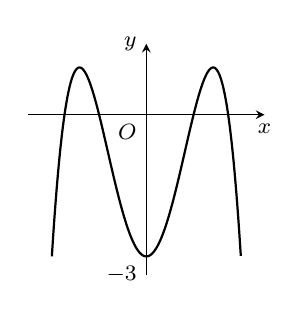
\begin{tikzpicture}[>=stealth,x=1cm,y=1cm,scale=.6,font=\footnotesize ]
	\def\a{-1} % Hệ số a phải khác 0
	\def\b{4}
	\def\c{-3}
	\draw[->] (-2.5,0) -- (2.5,0) node[below] {$x$};
	\draw[->] (0,-3.4) -- (0,1.5) node[left] {$y$};
	\draw (0,0)node[below left]{$O$};
	\draw[thick,samples=150,smooth,domain=-2:2] plot(\x,{\a*(\x)^4+(\b)*(\x)^2+(\c)});
	\path (0,-3)node[below left]{$ -3 $};
	\end{tikzpicture}
	}
	\loigiai{
	Ta có $\lim\limits_{x\to\pm\infty} y=-\infty$ nên $a<0$.\\
	Khi $x=0$ suy ra $y=c$. \\
	Đồ thị cắt trục $ Oy $ tại $y=-3\Rightarrow c=-3<0$.\\
	Ta có $y'=4ax^3+2bx=0\Leftrightarrow\hoac{&x=0\\&x^2=-\dfrac{b}{2a}.}$ \\
	Đồ thị hàm số có 3 cực trị nên $-\dfrac{b}{2a}>0\Rightarrow ab<0\Rightarrow b>0$.}
\end{ex}
%%==========Câu 20
\begin{ex}%[2D2B3-3]
	Nếu $a^{\tfrac{\sqrt{3}}{3}}>a^{\tfrac{\sqrt{2}}{2}}$ và $\log_b\left(\dfrac{3}{4}\right)<\log_b\left(\dfrac{4}{5}\right)$ thì
	\choice
	{\True $0<a<1$, $ b>1$}
	{$0<b<1$, $ a>1$}
	{$a>1$, $ b>1$}
	{$0<a<1$, $ 0<b<1$}
	\loigiai{
	Do $\dfrac{\sqrt{3}}{3}<\dfrac{\sqrt{2}}{2}$ và $a^{\tfrac{\sqrt{3}}{3}}>a^{\tfrac{\sqrt{2}}{2}}$ nên suy ra $0<a<1$. \\
	Do $\dfrac{3}{4}<\dfrac{4}{5}$ và $\log_b\left(\dfrac{3}{4}\right)<\log_b\left(\dfrac{4}{5}\right)$ nên suy ra $b>1$.}
\end{ex}
%%==========Câu 21
\begin{ex}%[2D2K4-3]
	\immini
	{
	Cho các hàm số $y=\log_ax$, $ y=b^x$, $ y=c^x$ có đồ thị như hình bên. Chọn khẳng định đúng.
	\choice
	{$c>b>a$}
	{$a>b>c$}
	{\True $b>c>a$}
	{$b>a>c$}
	}
	{
	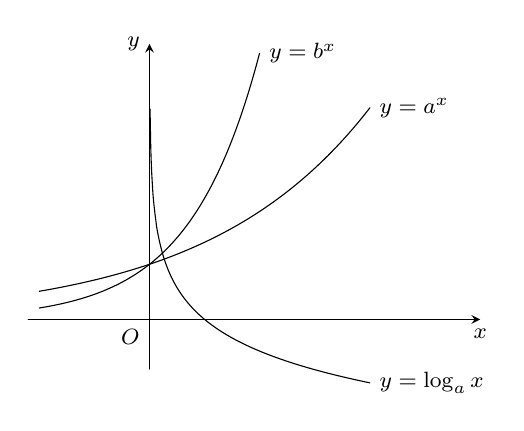
\begin{tikzpicture}[scale=.7,>=stealth, font=\footnotesize, line join=round, line cap=round]
	\def\xmin{-2.2} \def\xmax{6} \def\ymax{5}
	\draw[->] (\xmin,0)--(\xmax,0) node [below]{$x$};
	\draw[->] (0,-0.9)--(0,\ymax) node [left]{$y$};
	\node at (0,0) [below left]{$O$};
	\draw[smooth,samples=300,domain=-2:2] plot(\x,{2.2^(\x)})node[right]{$ y=b^x $};
	\draw[smooth,samples=300,domain=-2:4] plot(\x,{1.4^(\x)})node[right]{$ y=a^x $};
	\draw[smooth,samples=300,domain=0.01:4] plot(\x,{ln(\x)/ln(0.3)})node[right]{$ y=\log_ax $};
	\end{tikzpicture}
	}
	\loigiai{
	Dựa vào đồ thị ta suy ra $0<a<1; b, c>1$.\\
	Dựa vào giao điểm của đường thẳng $x=1$ với các đồ thị hàm số $y=b^x$, $ y=c^x$ ta suy ra $c<b$.\\
	Vậy $b>c>a$.}
\end{ex}
%%==========Câu 22
\begin{ex}%[2D2B6-2]
	Tập nghiệm của bất phương trình $\left(\dfrac{1}{2}\right)^{x^2-2}>2^{4-3x}$ là
	\choice
	{$(-\infty; 1)$}
	{$(2;+\infty)$}
	{\True $(1; 2)$}
	{$(-\infty; 1)\cup(2;+\infty)$}
	\loigiai{
	Ta có $\left(\dfrac{1}{2}\right)^{x^2-2}>2^{4-3x}\Leftrightarrow 2^{2-x^2}>2^{4-3x}$\\
	$ \Leftrightarrow 2-x^2>4-3x\Leftrightarrow x^2-3x+2<0\Leftrightarrow 1<x<2 $.\\
	Vậy $x\in(1; 2)$.}
\end{ex}
%%==========Câu 23
\begin{ex}%[2D3B1-2]
	Tìm nguyên hàm $F(x)=\displaystyle\int\sin^22x\mathrm{\,d}x$
	\choice
	{$F(x)=\dfrac{1}{2}x-\dfrac{1}{8}\cos 4x+C$}
	{\True $F(x)=\dfrac{1}{2}x-\dfrac{1}{8}\sin 4x+C$}
	{$F(x)=\dfrac{1}{2}x-\dfrac{1}{8}\sin 4x$}
	{$F(x)=\dfrac{1}{2}x+\dfrac{1}{8}\sin 4x+C$}
	\loigiai{
	Ta có $F(x)=\displaystyle\int\sin^22x\mathrm{\,d}x=\displaystyle\int\dfrac{1-\cos 4x}{2}\mathrm{\,d}x=\dfrac{1}{2}\displaystyle\int 1\mathrm{\,d}x-\dfrac{1}{2}\displaystyle\int\cos 4x\mathrm{\,d}x$\\
	$=\dfrac{1}{2}x-\dfrac{1}{8}\displaystyle\int\cos 4x\mathrm{d}(4x)=\dfrac{1}{2}x-\dfrac{1}{8}\sin 4x+C$.}
\end{ex}
%%==========Câu 24
\begin{ex}%[2D4K3-2]
	Cho số phức z thỏa mãn $(2-i)z+\dfrac{1+5i}{1+i}=7+10i$. Mô-đun của số phức $w=z^2+20+3i$ là
	\choice
	{\True $ 5 $}
	{$ 3 $}
	{$ 25 $}
	{$ 4 $}
	\loigiai{
	Ta có $(2-i)z+\dfrac{1+5i}{1+i}=7+10i\Leftrightarrow(2-i)z+3+2i=7+10i\Leftrightarrow(2-i)z=4+8i$.\\
	Suy ra $z=\dfrac{4+8i}{2-i}=4i$ nên $w=(4i)^2+20+3i=4+3i$. \\
	Vậy $|w|=5$.}
\end{ex}
%%==========Câu 25
\begin{ex}%[2D4K1-2]
	Tập hợp các điểm biểu diễn số phức z thỏa mãn $\left|\dfrac{\overline{z}}{3}+1+2i\right|=5$ là
	\choice
	{\True Đường tròn tâm $I(-3; 6)$, bán kính $R=15$}
	{Đường tròn tâm $I(-3; 6)$, bán kính $R=5$}
	{Đường tròn tâm $I(-1; 2)$, bán kính $R=5$}
	{Đường tròn tâm $I(3;-6)$, bán kính $R=15$}
	\loigiai{
	Gọi $z=x+yi$, $ x$, $ y\in \mathbb{R}$ thì $\overline{z}=x-yi$, $\dfrac{\overline{z}}{3}=\dfrac{x}{3}-\dfrac{y}{3}i$.\\
	Vậy $\left|\dfrac{\overline{z}}{3}+1+2i\right|=\left|\left(\dfrac{x}{3}+1\right)+\left(2-\dfrac{y}{3}\right)i\right|$.\\
	Suy ra $\left(\dfrac{x}{3}+1\right)^2+\left(2-\dfrac{y}{3}\right)^2=5^2 \Leftrightarrow(x+3)^2+(y-6)^2=15^2 $.\\
	Vậy điểm biểu diễn số phức $ z $ nằm trên đường tròn tâm $I(-3; 6)$, bán kính $R=15$.}
\end{ex}
\begin{ex}%[2H1Y3-2]%Câu 26.
	Khối chóp $S.ABC$ có $SA$ vuông góc với đáy, $SBC$ là tam giác đều cạnh $a$, tam giác $ABC$ vuông tại $A$. Thể tích của khối chóp $S.ABC$ bằng
	\choice
	{$\dfrac{\sqrt{2}}{12}a^3$}
	{\True $\dfrac{\sqrt{2}}{24}a^3$}
	{$\dfrac{\sqrt{2}}{32}a^3$}
	{$\dfrac{\sqrt{2}}{36}a^3$}
	\loigiai{
		\immini{
			$\Delta SAB=\Delta SAC$ (cạnh huyền – cạnh góc vuông) nên suy ra $AB=AC$ mà $\Delta ABC$ lại vuông tại A nên nó là tam giác vuông cân tại A do đó $AB=AC=\dfrac{BC}{\sqrt{2}}=\dfrac{a}{\sqrt{2}}$.\\
			$\Delta SAB$ vuông tại A nên $SA=\sqrt{SB^2-AB^2}=\dfrac{a}{\sqrt{2}}$.\\
			Thể tích khối chóp S. ABC là 
			\[V=\dfrac{1}{3}\cdot\dfrac{1}{2}\cdot AB\cdot AC\cdot SA=\dfrac{1}{6}\left(\dfrac{a}{\sqrt{2}}\right)^3=\dfrac{\sqrt{2}}{24}a^3.\]}
		{
			\begin{tikzpicture}[scale=1, font=\footnotesize, line join=round, line cap=round, >=stealth]
			\path 
			(0,0) coordinate (A)
			(3,0) coordinate (B)
			(1.7,-1.2) coordinate (C)
			(0,2) coordinate (S)
			;
			\draw 
			(S)--(A)--(C)--($(C)!.5!(B)$) node[below right] {$a$}--(B)--($(S)!.5!(B)$) node[above right] {$a$}--(S)--($(S)!.5!(C)$) node[right] {$a$}--(C);
			\draw[dashed] (A)--(B)
			;
			\draw pic[draw,angle radius=2mm]{right angle=S--A--B};
			\draw pic[draw,angle radius=2mm]{right angle=S--A--C};
			\draw pic[draw,angle radius=2mm]{right angle=C--A--B};
			\foreach \x/\g in {S/90,A/-135,C/-90,B/-45} \fill[black](\x) circle (1pt) ($(\x)+(\g:3mm)$) node{\x};
			\end{tikzpicture}
		}
	}
\end{ex}
\begin{ex}%[2H2B2-6]%Câu 27.
	Cho tam giác $ABC$ đều cạnh $a$. Quay tam giác $ABC$ quanh đường cao $AH$ ta được hình nón tròn xoay. Diện tích mặt cầu nội tiếp hình nón bằng
	\choice
	{$\dfrac{\pi a^2}{2}$}
	{\True $\dfrac{\pi a^2}{3}$}
	{$\pi a^2$}
	{$2\pi a^2$}
	\loigiai{
		\immini{
			Mặt cầu nội tiếp hình nón có $1$ đường tròn lớn nội tiếp tam giác đều $ABC$ (cạnh $a$).\\
			Nên mặt cầu đó có bán kính $r=\dfrac{1}{3}\cdot\dfrac{a\sqrt{3}}{2}=\dfrac{a\sqrt{3}}{6}$.\\
			Vậy diện tích mặt cầu cần tìm là
			\[V=4\pi r^2=4\pi\left(\dfrac{a\sqrt{3}}{6}\right)^2=\dfrac{\pi a^2}{3}.\]}
		{\begin{tikzpicture}[scale=.7, font=\footnotesize, line join=round, line cap=round, >=stealth]
			\def\x{3} % Bán kính trụ lớn
			\pgfmathsetmacro{\y}{\x/4} % Bán kính trục bé
			\def\z{1.5} % Bán kính trụ lớn
			\pgfmathsetmacro{\t}{\z/3} % Bán kính trục bé
			\def\h{5} % Chiều cao
			\coordinate[label=below:$O$] (O) at (0,0);
			\coordinate[label=right:$C$] (C) at (\x,0);
			\coordinate[label=above:$A$] (A) at (0,\h);
			\coordinate[label=left:$B$] (B) at ($(C)!2!(O)$); % Định nghĩa điểm M thỏa mãn \vt{AM}=1/2*\vt{AB}
			\tkzInCenter(A,B,C) \tkzGetPoint{I}
			\tkzDrawCircle[radius,dashed](I,O) 
			\tkzInterLC(A,C)(I,O) \tkzGetPoints{a}{a} 
			\draw (C) arc (0:-180:{\x} and {\y})--(A)--cycle;
			\draw[dashed] (A)--(O) (B)--(C) arc (0:180:{\x} and {\y});
			\draw (a) arc (0:-180:{\z} and {\t});
			\draw[dashed] (a) arc (0:180:{\z} and {\t});
			\foreach \diem in {C,A,O}	\fill (\diem)circle(1pt);
			\end{tikzpicture}}}
\end{ex}
\begin{ex}%[2H3Y2-3]%Câu 28.
	Trong không gian với hệ trục tọa độ $Oxyz$, cho hai điểm $A(-2; 1; 4)$, $B(4; 3;-2)$. Viết phương trình mặt phẳng trung trực của đoạn thẳng $AB$. 
	\choice
	{$3x+y+3z-8=0$}
	{\True $3x+y-3z-2=0$}
	{$3x+y-3z-8=0$}
	{$6x+2y-6z-2=0$}
	\loigiai{
		Gọi $I$ là trung điểm của $AB \Rightarrow I(1; 2;1)$.\\
		Giả sử $(P)$ là mặt phẳng trung trực của đoạn $AB \Rightarrow \heva{&I\in(P)\\&\overrightarrow{n}_P=\overrightarrow{AB}=(6; 2;-6)=2(3; 1;-3).}$ \\
		Vậy phương trình mặt phẳng $(P)\colon 3x+y-3z-2=0$.}
\end{ex}
\begin{ex}%[2H3Y2-6]%Câu 29.
	Trong không gian $Oxyz$, khoảng cách giữa hai mặt phẳng $(P)\colon x+2y+2z-10=0$ và $(Q)\colon x+2y+2z-3=0$ bằng
	\choice
	{$\dfrac{8}{3}$}
	{\True $\dfrac{7}{3}$}
	{3}
	{$\dfrac{4}{3}$}
	\loigiai{
		Xét thấy $(P)$ và $(Q)$ là hai mặt phẳng song song với nhau.\\
		\textbf{Cách 1:} Trên $(P)$ lấy $M(0; 0; 5)$.\\
		Khi đó, khoảng cách giữa hai mặt phẳng $(P)$ và $(Q)$ là
		\[\mathrm{d}\left((P),(Q)\right)=\mathrm{d}\left(M,(Q)\right)=\dfrac{\left|0+2\cdot 0+2\cdot 5-3\right|}{\sqrt{1^2+2^2+2^2}}=\dfrac{7}{3}.\]
		\textbf{Cách 2.}
		$(P)\colon Ax+By+Cz+D=0$ và $(P')\colon Ax+By+Cz+D'=0$.\\
		Thì $\mathrm{d}\left((P),(P')\right)=\dfrac{|D-D'|}{\sqrt{A^2+B^2+C^2}}$.\\
		Áp dụng $\mathrm{d}\left((P),(Q)\right)=\dfrac{\left|-10-(-3)\right|}{\sqrt{1^2+2^2+2^2}}=\dfrac{7}{3}$.
	}
\end{ex}
\begin{ex}%[1H3B3-3]%Câu 30.
	Cho lăng trụ tam giác đều $ABC.A'B'C'$ có cạnh đáy bằng $a$, cạnh bên bằng $2a$. Gọi $M$ là trung điểm của $AA'$. Gọi góc giữa đường thẳng $MB'$ và mặt phẳng $(BCC'B')$ là $\alpha$, góc $\alpha$ thỏa mãn đẳng thức nào dưới đây?
	\choice
	{\True $\sin\alpha=\dfrac{\sqrt{6}}{4}$}
	{$\sin\alpha=-\dfrac{\sqrt{6}}{4}$}
	{ $\cos\alpha=\dfrac{\sqrt{6}}{4}$}
	{$\sin\alpha=\dfrac{\sqrt{3}}{2}$}
	\loigiai{
		\immini{
			Gọi $J$ là trung điểm của $BC \Rightarrow AJ\perp(BCC'B')$,
			tam giác $ABC$ đều cạnh $a$ nên $AJ=\dfrac{a\sqrt{3}}{2}$;       $MB'=a\sqrt{2}$.\\
			Ta có:\\
			$\sin\left(MB',(BCC'B')\right)=\dfrac{\mathrm{d}\left(M;(BCC'B')\right)}{MB'}=\dfrac{\mathrm{d}\left(A;(BCC'B')\right)}{MB'}=\dfrac{AJ}{MB'}=\dfrac{\sqrt{6}}{4}$.
		}
		{
			\begin{tikzpicture}[scale=1, font=\footnotesize, line join=round, line cap=round, >=stealth]
			\def\h{3}
			\def\a{3}
			\def\b{1}
			\def\c{1.2}
			\path
			(0,0) coordinate (A')
			(\a,0) coordinate (C')
			(\b,-\c) coordinate (B')
			($(A')+(0,\h)$) coordinate (A)
			($(B')+(0,\h)$) coordinate (B)
			($(C')+(0,\h)$) coordinate (C)
			($(A)!.5!(A')$) coordinate (M)
			($(B)!.5!(C)$) coordinate (J)
			;
			\draw 
			(B)--(C)--(C')--(B')--(A')--(A)--(B)--(B')
			(C)--(A)--(J)
			;
			\draw[dashed] (A')--(C');
			\foreach \x/\g in {A/135,B/80,C/45,A'/-135,B'/-90,C'/-45,J/-45,M/180} \fill[black](\x) circle (1pt) ($(\x)+(\g:3mm)$) node{\x};
			\end{tikzpicture}	
		}
	}
\end{ex}
\begin{ex}%[1D2Y5-4]%Câu 31.
	Một nhóm học sinh gồm có $4$ nam và $5$ nữ, chọn ngẫu nhiên ra $2$ bạn. Tính xác suất để $2$ bạn được chọn có $1$ nam và $1$ nữ. 
	\choice
	{$\dfrac{4}{9}$}
	{$\dfrac{5}{18}$}
	{\True $\dfrac{5}{9}$}
	{$\dfrac{7}{9}$}
	\loigiai{
		Chọn $2$ học sinh trong $9$ học sinh có $\mathrm{C}_9^2$ cách $\Rightarrow n(\Omega)=\mathrm{C}_9^2$.\\
		Gọi $A$ là biến cố \lq\lq $2$ học sinh được chọn có $1$ nam và $1$ nữ \rq\rq $\Rightarrow n(A)=\mathrm{C}_4^1\cdot\mathrm{C}_5^1$.\\
		Xác suất cần tìm là $\mathrm{P}(A)=\dfrac{\mathrm{C}_4^1\cdot\mathrm{C}_5^1}{\mathrm{C}_9^2}=\dfrac{5}{9}$.
	}
\end{ex}
\begin{ex}%[2D1K3-1]%Câu 32.
	\immini{
		Cho hàm số $y=f(x)$. Đồ thị $y=f'(x)$ như hình bên.\\
		Biết $f(-1)+f(0)-2f(1)=f(3)-f(2)$. Giá trị nhỏ nhất của hàm số trên đoạn $[-1; 3]$ là
		\choice
		{$f(-1)$}
		{$f(0)$}
		{\True $f(3)$}
		{$f(2)$}
	}
	{
		\begin{tikzpicture}[>=stealth]
		\draw[->] (-1.5,0)--(0,0) node[below left]{$O$} -- (4,0)	node[below]{$x$};
		\draw[->] (0,-2.5)--(0,2)	node[left]{$y$};
		\draw[line width=0.5 pt,smooth] plot[domain=-1.05:3.1] (\x,{(1/4)*(\x)^3-(\x)^2-(1/4)*(\x) +1});
		\draw[dashed] (3,0)--(3,-2);
		\foreach \x/\g in {-1/-90,1/-90,3/90} 
		\draw (\x,-1pt)--(\x,1pt) ($(\x,0)+(\g:3mm)$) node {$\x$};
		\end{tikzpicture}	
	}
	\loigiai{
		Ta có bảng biến thiên của hàm số $y=f(x)$. 
		\begin{center}
			
\begin{tikzpicture}[>=stealth]
			\tkzTabInit[nocadre=false,lgt=1.2,espcl=2,deltacl=1.2]{$x$/0.6 ,$f'(x)$/.6,$f(x)$/2}
			{$-1$ , $1$ , $\sqrt{3}$}
			\tkzTabLine{$0$ , + , $0$ , - , }
			\tkzTabVar{-/$f(-1)$ ,+/$f(1)$ , -/$f(3)$}
			\end{tikzpicture}
		\end{center}
		Vậy $\max\limits_{[-1; 3]} f(x)=f(1)$.\\	
		Từ bảng biến thiên ta có $f(0)<f(1), f(2)<f(1)$ vậy $f(0)+f(2)<2f(1)$.\\
		Khi đó $f(-1)+f(0)-2f(1)=f(3)-f(2)\Leftrightarrow f(0)+f(2)-2f(1)=f(3)-f(-1)$.\\
		Vậy $f(3)-f(-1)<0\Rightarrow f(3)<f(-1)$.\\
		Khi đó $\min\limits_{[-1; 3]} f(x)=f(3)$.}
\end{ex}
\begin{ex}%Câu 33.%[1D1K2-6]
	Cho hàm số $y=(m+1)x^4-2x^2+1$ (với $m$ là tham số). Tìm tất cả các giá trị thực của $m$ để hàm số đã cho có ba điểm cực trị đều nhỏ hơn $1$. 
	\choice
	{$-1<m<0$}
	{$m >-1$}
	{$0<m<1$}
	{\True $m>0$}
	\loigiai{
		Trường hợp 1. Nếu $m+1=0 \Leftrightarrow m=-1$ thì hàm số đã cho trở thành $y=2x^2+1$, hàm số này có một điểm cực trị, do đó ta loại trường hợp này.\\
		Trường hợp 2. Nếu $m+1 \ne 0 \Leftrightarrow m \ne -1$.\\
		Ta có $y' = 4(m+1)x^3-4x = 4x \left[(m+1)x^2-1\right]$.\\
		$y'=0 \Leftrightarrow \hoac{&x=0 \\ &(m+1)x^2-1=0} \Leftrightarrow \hoac{&x=0 \\ &x^2=\dfrac{1}{m+1} \quad (1).}$ \\
		Hàm số đã cho có ba điểm cực trị đều nhỏ hơn 1 khi phương trình (1) có hai nghiệm phân biệt khác 0 và nhỏ hơn 1.
		Hay $0 < \dfrac{1}{m+1} < 1 \Leftrightarrow \heva{ &\dfrac{1}{m+1} > 0 \\ &\dfrac{1}{m+1} < 1} \Leftrightarrow \heva{&\dfrac{1}{m+1} > 0 \\ &\dfrac{-m}{m+1} < 0} \Leftrightarrow \heva{&m >-1 \\ &\hoac{&m<-1 \\ &m>0}} \Leftrightarrow m>0$.}
%<MyLT>
\end{ex}
\begin{ex}%Câu 34.%[2D2K5-3]
	Tìm $m$ để phương trình $-\log_2^3x+m\log_2x+2=0$ có nghiệm duy nhất. 
	\choice
	{\True $m<3$}
	{$m \le 3$}
	{$m>0$}
	{$m \ge 0$}
	\loigiai{
		Đặt $\log_2 x = t$, ta được phương trình $-t^3+mt+2 = 0$, $t\in \mathbb{R}$.\\
		Để phương trình $-\log_2^3{x} + m\log_2 {x} +2 = 0$ có nghiệm duy nhất khi và chỉ khi phương trình $-t^3+mt+2=0$, $t\in \mathbb{R}$ có nghiệm duy nhất.\\
		Ta thấy $t=0$ không là nghiệm của phương trình $-t^3+mt+2=0$.\\
		Khi đó $-t^3+mt+2=0 \Leftrightarrow m=\dfrac{t^3-2}{t}=t^2-\dfrac{2}{t}$.\\
		Số nghiệm phương trình là số giao điểm của đồ thị $y=f(t)=t^2-\dfrac{2}{t}$ và đường thẳng $y=m.$ \\
		$f'(t) = 2t + \dfrac{2}{t^2} = \dfrac{2t^3+2}{t^2} = 0 \Rightarrow t=-1$.\\
		\begin{center}
			
\begin{tikzpicture}[>=stealth]
			\tkzTabInit[nocadre=false,lgt=1,espcl=2,deltacl=0.5]{$t$/.8 ,$f'(t)$/.8,$f(t)$/2}
			{$-\infty$ , $-1$ , $0$ , $+\infty$}
			\tkzTabLine{ , - , $0$ , + , d , + }
			\tkzTabVar{+/$+\infty$ , -/$3$ , +D-/$+\infty$/$-\infty$,+/$+\infty$}
			\end{tikzpicture}
		\end{center}	
		Dựa vào BBT, ta có $m<3$.\\
		Cách khác: Thử điểm cực biên ở mỗi phương án chọn, cụ thể thử với.\\
		$m=0; m=3; m=-1$.}
%<MyLT>
\end{ex}
\begin{ex}%Câu 35.%[2D1G3-6]
	\immini{
		Anh A có một mảnh đất bồi ven sông, anh muốn trồng cây trên mảnh đất này, để tính chi phí anh cho lên bản vẽ thì thấy mảnh đất có hình parabol như hình vẽ. Chiều cao $GH = 4$m, chiều rộng $AB = 4$m, $AC = BD = 0,9$m. Anh A dự định trồng rau ở phần hình chữ nhật $CDEF$ (tô màu), mua phân bón và cây giống là $50000$ $\text{đồng/m}^2$, còn các phần để trắng trồng cà chua có giá là $30000$ $\text{đồng/m}^2$. Hỏi tổng chi phí để hai phần nói trên gần nhất với số tiền nào dưới đây?
		\choice
		{\True $443000$ (đồng)}
		{$553500$ (đồng)}
		{$320000$ (đồng)}
		{$370000$ (đồng)}
	}{
		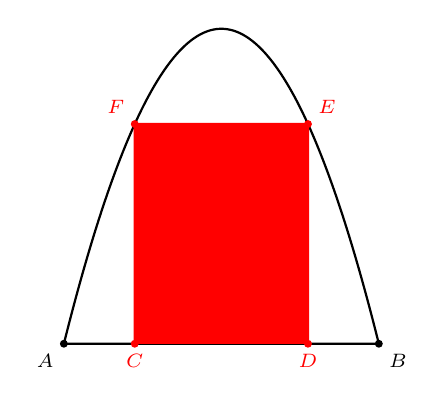
\begin{tikzpicture}[>=stealth,x=1cm,y=1cm,scale=1,font=\scriptsize,fill=black]
		\def\a{-1}
		\def\b{4}
		\def\c{0}
		\def\f(#1){\a*(#1)^2+\b*(#1)+\c}
		\draw[thick,fill] (0,0)circle(1pt)node[below left]{$A$} -- (4,0)circle(1pt)node[below right]{$B$};
		\draw[thick,samples=150,smooth,domain=0:4] plot(\x,{\f(\x)});
		\draw[red,thick,fill] (0.9,0)circle(1pt) node[below]{$C$} 
		-- (0.9,{\f(0.9)})circle(1pt)node[above left]{$F$} 
		-- (3.1,{\f(3.1)})circle(1pt)node[above right]{$E$}
		-- (3.1,0)circle(1pt)node[below]{$D$};
		\fill[red] (0.9,0)rectangle(3.1,{\f(3.1)});
		\end{tikzpicture}}
	\loigiai{
		\immini{
			Gắn hệ trục tọa độ $Oxy$ sao cho $AB$ trùng với $Ox$, $A$ trùng $O$ khi đó parabol có đỉnh $G(2; 4)$ và đi qua gốc tọa độ.\\
			Gọi phương trình của parabol là $y=ax^2+bx+c$.\\
			Khi đó ta có $\heva{&c=0 \\ &\dfrac{-b}{2a}=2 \\ &2^2a+2b+c=4} \Leftrightarrow \heva{&a=-1 \\ &b=4 \\ &c=0.}$\\
			Nên phương trình parabol là $y=f(x)=-x^2+4x$.\\
			Diện tích của cả mảnh đất là $S=\displaystyle\int\limits_0^4 \left(-x^2+4x\right) \mathrm{\,d}x = \left(-\dfrac{x^3}{3}+2x^2\right)\bigg|_0^4 = \dfrac{32}{3} \approx 10,67(\text{m}^2)$.			
		}{
			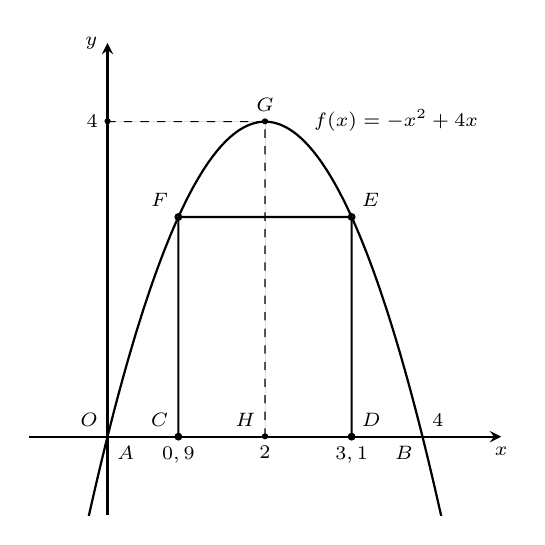
\begin{tikzpicture}[>=stealth,x=1cm,y=1cm,scale=1,font=\scriptsize,fill=black]
			\def\a{-1}
			\def\b{4}
			\def\c{0}
			\def\f(#1){\a*(#1)^2+\b*(#1)+\c}
			\draw[thick,->] (-1,0) -- (5,0) node[below] {$x$};
			\draw[thick,->] (0,-1) -- (0,5) node[left] {$y$};
			\draw (0,0)node[above left]{$O$} node[below right]{$A$} (4,0)node[below left]{$B$} node[above right]{$4$};
			\pgfmathsetmacro\xdinh{-(\b)/2*(\a)}
			\pgfmathsetmacro\ydinh{(4*(\a)*(\c)-(\b)^2)/(4*(\a))}
			\draw[dashed,fill] (\xdinh,0)circle(1pt)node[below]{$2$}node[above left]{$H$} 
			-- (\xdinh,\ydinh)circle(1pt)node[above]{$G$} 
			-- (0,\ydinh)circle(1pt)node[left]{$4$};
			\clip (-1,-1)rectangle(5,5);
			\draw[thick,samples=150,smooth,domain=-0.5:4.5] plot(\x,{\f(\x)});
			\draw[thick] (0.9,0)circle(1pt) node[below]{$0,9$}node[above left]{$C$} 
			-- (0.9,{\f(0.9)})circle(1pt)node[above left]{$F$} 
			-- (3.1,{\f(3.1)})circle(1pt)node[above right]{$E$}
			-- (3.1,0)circle(1pt)node[below]{$3,1$}node[above right]{$D$};
			\draw (2.5,{\f(2.5)})node[above right]{$f(x)=-x^2+4x$};
			\end{tikzpicture}}\noindent 
		Do vậy chiều cao $CF=DE=f(0,9)=2,79(\text{m})$; $CD=4-2\cdot 0,9=2,2(\text{m})$.\\
		Diện tích phần hình chữ nhật là $S_{CDEF}=CD\cdot CF=6,138\approx 6,14(\text{m}^2)$.\\
		Diện tích phần trồng cà chua là $S_{xh}=S-S_{CDEF}=10,67-6,14=4,53(\text{m}^2)$.\\
		Nên tiền trồng rau là $6,14\cdot 50000=307000$ và tiền trồng cà chua là $4,53\cdot 30000=136000$.\\
		Vậy tổng chi phí là $443000$ đồng.	
	}
%<MyLT>
\end{ex}
\begin{ex}%Câu 36.%[2D3T2-4]
	Cho hàm số $f(x)$ liên tục trên $\mathbb{R}$ đồng thời thỏa mãn $f(x)+f(-x)=3-2\cos x$, với mọi $x\in \mathbb{R}$. Tính tích phân $I=\displaystyle\int\limits_{-\tfrac{\pi}{2}}^{\tfrac{\pi}{2}} f(x)\mathrm{\,d}x$?
	\choice
	{$I=\dfrac{\pi}{2}+2$}
	{\True $I=\dfrac{3\pi}{2}-2$}
	{$I=\dfrac{\pi-1}{3}$}
	{$I=\dfrac{\pi+1}{2}$}
	\loigiai{
		Đặt $t=-x\Rightarrow\mathrm{\,d}t=-\mathrm{\,d}x$. Đổi cận $x=-\dfrac{\pi}{2}\Rightarrow t=\dfrac{\pi}{2}$; $x=\dfrac{\pi}{2}\Rightarrow t=-\dfrac{\pi}{2}$.\\
		Khi đó $I = -\displaystyle\int\limits_{\tfrac{\pi}{2}}^{-\tfrac{\pi}{2}} f(-t) \mathrm{\,d}t = \displaystyle\int\limits_{-\tfrac{\pi}{2}}^{\tfrac{\pi}{2}} f(-t) \mathrm{\,d}t = \displaystyle\int\limits_{-\tfrac{\pi}{2}}^{\tfrac{\pi}{2}} f(-x) \mathrm{\,d}x$.\\
		Mặt khác: $f(x)+f(-x) = 3-2\cos x$.\\
		Ta có: $2I = \displaystyle\int\limits_{-\tfrac{\pi}{2}}^{\tfrac{\pi}{2}} [f(x)+f(-x)] \mathrm{\,d}x = \displaystyle\int\limits_{-\tfrac{\pi}{2}}^{\tfrac{\pi}{2}} (3-2\cos x) \mathrm{\,d}x$\\
		$\Rightarrow I = \dfrac{1}{2} \displaystyle\int\limits_{-\tfrac{\pi}{2}}^{\tfrac{\pi}{2}} (3-2\cos x) \mathrm{\,d}x$.\\
		Do $f(x)=3-2\cos x$ là hàm số chẵn trên đoạn $\left[-\dfrac{\pi}{2} ; \dfrac{\pi}{2}\right]$.\\
		Nên $I = \dfrac{1}{2} \displaystyle\int\limits_{-\tfrac{\pi}{2}}^{\tfrac{\pi}{2}} (3-2\cos x) \mathrm{\,d}x = 2 \cdot \dfrac{1}{2} \displaystyle\int\limits_0^{\tfrac{\pi}{2}} (3-2\cos x) \mathrm{\,d}x = (3x-2\sin x) \bigg|_0^{\tfrac{\pi}{2}} = \dfrac{3\pi}{2}-2$.}
%<MyLT>
\end{ex}
\begin{ex}%Câu 37.%[2D4K2-4]
	Cho các số phức z thỏa mãn $(2+i)|z|=\dfrac{5}{z}-1-3i$. Biết rằng tập hợp các điểm biểu diễn các số phức $w=(3-4i)z+1$ là một đường tròn. Tính bán kính của đường tròn đó. 
	\choice
	{$r=25$}
	{$r=1$}
	{$r=\sqrt{5}$}
	{\True $r=5$}
	\loigiai{
		$(2+i)|z| = \dfrac{5}{z}-1-3i \Leftrightarrow (2+i)|z|+1+3i = \dfrac{5}{z}
		\Leftrightarrow (2|z|+1)+(|z|+3)i = \dfrac{5}{z} $.\\
		Lấy mô-đun 2 vế $\sqrt{(2|z|+1)^2+(|z|+3)^2} = \dfrac{5}{|z|}$.\\
		Đặt $|z|=t$, $t\geq 0$ khi đó ta có phương trình $t^4+2t^3+2t^2-5=0 \Leftrightarrow t=1 \Rightarrow |z|=1$.\\
		Khi đó $w=(3-4i)z+1 \Rightarrow w-1=(3-4i)z \Rightarrow |w-1|=\left|(3-4i)z\right| = \left|(3-4i)\right| \cdot |z|=5$.\\
		Vậy tập hợp các điểm biểu diễn cho số phức w là đường tròn tâm $I(1; 0); r=5$. }
%<MyLT>
\end{ex}
\begin{ex}%Câu 38.%[2H2T1-2]
	Một mặt cầu $(S)$ bán kính $R$. Một hình trụ có chiều cao $h$ và bán kính đáy bằng $r$ nội tiếp trong mặt cầu. Tính $h$ và $R$ sao cho diện tích xung quanh hình trụ là lớn nhất. 
	\choice
	{\True $h=R\sqrt{2}$}
	{$h=\dfrac{R\sqrt{2}}{2}$}
	{$h=2R$}
	{$h=R$}
	\loigiai{
		\immini{
			Cắt hình trụ theo mặt phẳng qua trục của hình trụ, ta được hình chữ nhật $ABCD$, như hình vẽ. Ta thấy.\\
			$$4R^2=h^2+4r^2\geq 2\sqrt{4h^2r^2}=4hr$$
			$$ \Leftrightarrow 2\pi R^2\geq 2\pi hr\Leftrightarrow S_{xq}\leq 2\pi R^2 $$
			Dấu ”=” xảy ra khi $h=2r=R\sqrt{2}$ và diện tích xung quanh của mặt trụ lớn nhất là $2\pi R^2$.}
		{\begin{tikzpicture}
			\def\r{2.5}
			\def\g{45}
			\path 
			(0,0) coordinate (O)
			(\g:\r) coordinate (A)
			(180-\g:\r) coordinate (B)
			(180+\g:\r) coordinate (C)
			(-\g:\r) coordinate (D)
			;
			\draw[dashed] 
			(B) arc (180:0:{\r*cos{\g}} and {0.2*\r*cos{\g}})
			(C) arc (180:0:{\r*cos{\g}} and {0.2*\r*cos{\g}})
			(A)--(B)--(C)--(D)--(A)--(C)
			($(A)!.5!(B)$)--($(C)!.5!(D)$);
			\draw
			(0,0) circle (\r)
			(B) arc (-180:0:{\r*cos{\g}} and {0.17*\r*cos{\g}})
			(C) arc (-180:0:{\r*cos{\g}} and {0.17*\r*cos{\g}});
			\path
			($(A)!.25!(C)$) node[below] {$R$}
			($(A)!.5!(D)$) node[right] {$h$}
			($(A)!.3!(B)$) node[above] {$r$}
			;
			\foreach \x/\g in {A/30,B/150,C/210,D/-30} \fill[black](\x) circle (1pt) ($(\x)+(\g:3mm)$) node{\x};
			\end{tikzpicture}}}
%<MyLT>
\end{ex}

\begin{ex}%Câu 39.%[2H3T3-2]
	Trong không gian với hệ tọa độ $Oxyz$, cho hai đường thẳng $d_1\colon\dfrac{x-2}{-1}=\dfrac{y-1}{3}=\dfrac{z-1}{2}$ và $d_2\colon\heva{&x=1-3t\\&y=-2+t\\&z=-1-t}$. Phương trình đường thằng nằm trong $(\alpha)\colon x+2y-3z-2=0$ và cắt hai đường thẳng $d_1, d_2$ là
	\choice
	{\True $\dfrac{x-3}{-5}=\dfrac{y+2}{1}=\dfrac{z+1}{-1}$}
	{$\dfrac{x+3}{5}=\dfrac{y-2}{-1}=\dfrac{z-1}{1}$}
	{$\dfrac{x+3}{-5}=\dfrac{y-2}{1}=\dfrac{z-1}{-1}$}
	{$\dfrac{x+8}{1}=\dfrac{y-3}{3}=\dfrac{z}{-4}$}
	\loigiai{
		Gọi $d$ là đường thẳng cần tìm.
		\begin{itemize}
			\item Gọi $A=d_1\cap(\alpha)$.\\
			$A\in d_1\Rightarrow A\left(2-a; 1+3a; 1+2a\right)$.\\
			$A\in(\alpha)\Rightarrow a=-1\Rightarrow A(3;-2;-1)$.
			\item Gọi $B=d_2\cap(\alpha)$.\\
			$B\in d_2\Rightarrow B\left(1-3b;-2+b;-1-b\right)$.\\
			$B\in(\alpha)\Rightarrow b=1\Rightarrow B(-2;-1;-2)$.
			\item $d$ đi qua điểm $A(3;-2;-1)$ và có véc-tơ chỉ phương $\overrightarrow{AB}=(-5; 1;-1)$.
		\end{itemize}
		Vậy phương trình chính tắc của $d$ là $\dfrac{x-3}{-5}=\dfrac{y+2}{1}=\dfrac{z+1}{-1}$.}
%<MyLT>
\end{ex}
\begin{ex}%Câu 40.%[2H1G3-4]
	Cho hình chóp $S.ABCD$ có đáy $ABCD$ là hình vuông $BD=2a$, $\Delta SAC$ vuông tại $S$ và nằm trong mặt phẳng vuông góc với đáy, $SC=a\sqrt{3}$. Khoảng cách từ điểm $B$ đến mặt phẳng $(SAD)$ là
	\choice
	{$\dfrac{a\sqrt{30}}{5}$}
	{\True $\dfrac{2a\sqrt{21}}{7}$}
	{$2a$}
	{$a\sqrt{3}$}
	\loigiai{
		\immini{
			$\Delta SAC$ 
			vuông tại $S$ và nằm trong mặt phẳng vuông góc với đáy, nên kẻ $SH\perp AC\Rightarrow SH\perp(ABCD)$.\\
			$BD=AC=2a,CD=\dfrac{BD}{\sqrt{2}}=a\sqrt{2}$\\ $SA=\sqrt{AC^2-SC^2}=a$.\\
			$SH=\dfrac{SA\cdot SC}{AC}=\dfrac{a\cdot a\sqrt{3}}{2a}=\dfrac{a\sqrt{3}}{2}$.\\
			$AH=\sqrt{SA^2-SH^2}=\sqrt{a^2-\dfrac{3a^2}{4}}=\dfrac{a}{2}$.\\
			Gọi $O$ là tâm của hình vuông $ABCD$.\\
			Ta có $\mathrm{d}\left(B,(SAD)\right)=2\mathrm{d}\left(O,(SAD)\right)=4\mathrm{d}\left(H,(SAD)\right)$.\\
		}{\begin{tikzpicture}[scale=1, font=\scriptsize, line join=round, line cap=round, >=stealth]
			\def\bc{4} % cạnh BC
			\def\ba{2} % cạnh BA
			\def\h{4} % đường cao
			\def\gocB{30} % góc B của đáy
			\coordinate[label=below left:$B$] (B) at (0,0);
			\coordinate[label=above left:$A$] (A) at (\gocB:\ba);
			\coordinate[label=below:$C$] (C) at (\bc,0);
			\coordinate[label=right:$D$] (D) at ($(C)-(B)+(A)$);
			\coordinate[label=below left:$H$] (H) at ($(A)!1/4!(C)$); 
			\coordinate[label=above:$S$] (S) at ($(H)+(90:\h)$);
			\coordinate[label=below:$O$] (O) at ($(A)!1/2!(C)$); 
			\coordinate[label=above right:$J$] (J) at ($(A)!1/4!(D)$); 
			\coordinate[label=right:$K$] (K) at ($(J)!1/4!(S)$);
			\coordinate[label=below:$2a$] (a) at ($(O)!1/2!(D)$);
			\draw (B)--(C)--(D)--(S)--cycle (S)--(C) ;
			\draw[dashed] (A)--(D) (S)--(A)--(B) (S)--(H) (A)--(C) (B)--(D) (S)--(J) (H)--(K) (H)--(J);
			\foreach \diem in {A,B,C,D,S,H,O,J,K}	\fill (\diem)circle(1pt);
			\newcommand{\gocv}[4][black]{\draw[#1] ($(#3)!5pt!(#2)$)--($(#3)!2!($($(#3)!5pt!(#2)$)!.5!($(#3)!5pt!(#4)$)$)$)--($(#3)!5pt!(#4)$);}
			\gocv{S}{H}{C} \gocv{B}{A}{D}
			\end{tikzpicture}}\noindent 
		Kẻ $HJ\parallel CD(J\in AD), HJ=\dfrac{1}{4}CD=\dfrac{a\sqrt{2}}{4}$. Kẻ $HK\perp SJ$ tại K $\Rightarrow HK\perp(SAD)$ \\
		$ \Rightarrow\mathrm{d}\left(B,(SAD)\right)=4HK=4\cdot\dfrac{SH\cdot HJ}{\sqrt{SH^2+HJ^2}}=4\cdot\dfrac{\dfrac{a\sqrt{3}}{2}\dfrac{a\sqrt{2}}{4}}{\sqrt{\dfrac{3a^2}{4}+\dfrac{2a^2}{16}}}=\dfrac{2a\sqrt{21}}{7} $.}
%<MyLT>
\end{ex}
\begin{ex}%Câu 41.%[2D1G1-3]
	\immini{
		Cho hàm số $y=f(x)$ có đồ thị như hình vẽ bên.
		Có tất cả bao nhiêu giá trị nguyên của tham số $m$ thuộc khoảng $\left(-2020; 2020\right)$ để hàm số $y=f\left(\cos x+2x+m\right)$ đồng biến trên nửa khoảng $[0;+\infty)$. 
		\choice
		{\True $2019$}
		{$2020$}
		{$4038$}
		{$4040$}}
	{% Đồ thị hàm y=ax^3+bx^2+cx+d. Nếu hệ số lớn cần điều chỉnh hệ trục, vùng lưới, domain và lệnh \clip
		\begin{tikzpicture}[>=stealth,x=1cm,y=1cm,scale=0.8]
		\draw (0,0)node[below left]{\scriptsize $O$};
		\clip (-2.5,-2.5)rectangle(4.5,5.5);
		\draw[->] (-5,0)--(4,0)node[below]{$x$};
		\foreach \x in {-1,1,2}
		\draw[shift={(\x,0)}] (0,2pt)--(0,-2pt) node[below]{\scriptsize $\x$};
		\draw[->] (0,-5)--(0,5)node[right]{$y$};
		\foreach \y in {-2,-1,1,2,3}
		\draw[shift={(0,\y)}] (2pt,0)--(-2pt,0) node[right]{\scriptsize $\y$};
		\draw[thick,samples=150,smooth,domain=-1.2:3.2] plot(\x,{(0.75)*(\x)^3-(2.25)*(\x)^2+3});		
		\end{tikzpicture}		
	}
	\loigiai{
		Ta có $y'=(-\sin x+2)\cdot f'\left(\cos x+2x+m\right)$.\\
		Hàm số $y=f\left(\cos x+2x+m\right)$ liên tục trên nửa khoảng $[0;+\infty)$ \\
		$ \Rightarrow $ Hàm số $y=f\left(\cos x+2x+m\right)$ đồng biến trên $[0;+\infty)$ khi và chỉ khi\\
		$(-\sin x+2)\cdot f'\left(\cos x+2x+m\right)\geq 0,\forall x\in(0;+\infty)$ (1).\\
		Do $-\sin x+2>0,\forall x\in \mathbb{R}$ nên $(1)\Leftrightarrow f'\left(\cos x+2x+m\right)\geq 0,\forall x\in(0;+\infty)$ (2).\\
		Dựa vào đồ thị ta có\\
		$(2)\Leftrightarrow\hoac{&\cos x+2x+m\geq 2,\forall x\in(0;+\infty)\\&\cos x+2x+m\leq 0,\forall x\in(0;+\infty)}\Leftrightarrow\hoac{&\cos x+2x\geq 2-m,\forall x\in(0;+\infty) (3)\\&\cos x+2x\leq-m,\forall x\in(0;+\infty) (4).}$ \\
		Xét hàm $g(x)=\cos x+2x$ trên $[0;+\infty)$ có $g'(x)=-\sin x+2>0,\forall x\in(0;+\infty)$ nên $g(x)$ đồng biến trên $(0;+\infty)$ đồng thời $g(x)$ liên tục trên $[0;+\infty)$.\\
		Suy ra $\min\limits_{[0;+\infty)} g(x)=g(0)=1$ và $\lim\limits_{x\to+\infty} g(x)=+\infty$.\\
		Do đó, không có giá trị $m$ thỏa mãn (4).\\
		$(3)\Leftrightarrow\min\limits_{[0;+\infty)} g(x)\geq 2-m\Leftrightarrow 1\geq 2-m\Leftrightarrow m\geq 1$.\\
		Vậy có tất cả $2019$ giá trị nguyên của tham số $m$.}
%<MyLT>
\end{ex}
\begin{ex}%Câu 42.%[2D1G1-4]
	Có bao nhiêu giá trị nguyên của tham số $m$ thuộc đoạn $[-2018; 2018]$ để phương trình $\left(x+2-\sqrt{x^2+1}\right)^2+\dfrac{18\left(x^2+1\right)\sqrt{x^2+1}}{x+2+\sqrt{x^2+1}}=m\left(x^2+1\right)$ có nghiệm thực?
	\choice
	{$25$}
	{$2019$}
	{$2018$}
	{\True $2012$}
	\loigiai{
		Điều kiện $\heva{&x^2+1\geq 0\\&x+2+\sqrt{x^2+1}\neq 0}\Leftrightarrow x\in \mathbb{R}$ 
		\begin{center}
			
\begin{tikzpicture}[>=stealth]
			\tkzTabInit[nocadre=false,lgt=2,espcl=3,deltacl=1]{$x$/1 ,$t'$/.7,$t$/2}
			{$-\infty$ , $\dfrac{1}{2}$ , $+\infty$}
			\tkzTabLine{ , + , $0$ , - , }
			\tkzTabVar{-/$-1$ ,+/$\sqrt{5}$ , -/$1$}
			\end{tikzpicture}
		\end{center}
		Ta có $\left(x+2-\sqrt{x^2+1}\right)^2+\dfrac{18\left(x^2+1\right)\sqrt{x^2+1}}{x+2+\sqrt{x^2+1}}=m\left(x^2+1\right)$ \\
		$ \Leftrightarrow m=\left(\dfrac{x+2}{\sqrt{x^2+1}}-1\right)^2+\dfrac{18}{\dfrac{x+2}{\sqrt{x^2+1}}+1} $ .\\
		Đặt $t=\dfrac{x+2}{\sqrt{x^2+1}}\Rightarrow t'=\dfrac{1-2x}{\left(x^2+1\right)\sqrt{x^2+1}}$.\\
		Từ bảng biến thiên của $t$ suy ra $t\in(-1;\sqrt{5}]$.\\
		Phương trình trở thành $m=(t-1)^2+\dfrac{18}{t+1}\Leftrightarrow m=\dfrac{t^3-t^2-t+19}{t+1}$.\\
		$f(t)=\dfrac{t^3-t^2-t+19}{t+1}\Rightarrow f'(t)=\dfrac{2(t-2)\left(t^2+3t+5\right)}{(t+1)^2}$ \\
		Lập bảng biến thiên của $f(t)$ trên nửa khoảng $(-1;\sqrt{5}]$.\\
		\begin{center}
			
\begin{tikzpicture}[>=stealth]
			\tkzTabInit[nocadre=false,lgt=2,espcl=3,deltacl=1]{$t$/1 ,$f'(t)$/.7,$f(t)$/2}
			{$-1$ , $2$ , $\sqrt{5}$}
			\tkzTabLine{ , + , $0$ , - , }
			\tkzTabVar{+/$+\infty$ ,-/$7$ , +/$\dfrac{4\sqrt{5}+14}{\sqrt{5}+1}$}
			\end{tikzpicture}
		\end{center}
		Suy ta $f(t)\in[7;+\infty)$.\\
		Để phương trình.\\
		$\left(x+2-\sqrt{x^2+1}\right)^2+\dfrac{18\left(x^2+1\right)\sqrt{x^2+1}}{x+2+\sqrt{x^2+1}}=m\left(x^2+1\right)$.\\
		Có nghiệm thực thì $m\in[7;+\infty)$.\\
		Mà $m$ thuộc đoạn $[-2018; 2018]$ nên $m\in[7;2018]$.\\
		Có $2012$ giá trị nguyên của tham số $m$ thuộc đoạn $[-2018; 2018]$ để phương trình có nghiệm thực.}
%<MyLT>
\end{ex}
\begin{ex}%Câu 43.%[2D1G4-2]
	\immini{
		Cho hàm số $y=f(x)$ có đồ thị như hình vẽ dưới đây. Có bao nhiêu giá trị nguyên của tham số $m$ thuộc đoạn $[-20; 20]$ để đồ thị hàm số $y=f\left(x^2-2x+m\right)-m$ có $5$ đường tiệm cận?
		
		\choice
		{40}
		{\True 20}
		{21}
		{41}}
	{\begin{tikzpicture}[scale=0.7, font=\footnotesize, line join=round, line cap=round,>=stealth]
		\def\a{0} \def\b{1} \def\c{1} \def\d{0} % Hệ số
		\def\xmin{-4} \def\xmax{4}
		\def\ymin{-4} \def\ymax{4}
		%\draw[color=gray!50,dashed] (\xmin,\ymin) grid (\xmax,\ymax);
		\draw[->] (\xmin,0)--(\xmax,0) node [below]{$x$};
		\draw[->] (0,\ymin)--(0,\ymax) node [left]{$y$};
		\node at (0,0) [below left]{$O$};
		\clip (\xmin+0.1,\ymin+0.1) rectangle (\xmax-0.1,\ymax-0.1);
		\draw[smooth,samples=300,domain=\xmin+0.1:(-1-0.1)] plot(\x,{-1/((\x)^2-1)});
		\draw[smooth,samples=300,domain=(1+0.1:\xmax-0.1)]plot(\x,{1/((\x)^2-1)});
		\draw[smooth,samples=300,domain=-1:1]plot(\x,{-6*(\x)^3});
		\draw[dashed] (-1,\ymin)--(-1,\ymax);
		\draw[dashed] (1,\ymin)--(1,\ymax);
		\fill (0,0) circle (1.0pt) (-1,0) circle (1.0pt) node[above left]{$-1$} (1,0) circle (1.0pt) node[below right]{$1$};
		\end{tikzpicture}}
	\loigiai{
		Từ đồ thị hàm số $y=f(x)$ ta suy ra $f(x)$ có tập xác định $\mathscr{D}=\mathbb{R}\setminus\{\pm 1\}$ và các giới hạn $\lim\limits_{x\to\pm\infty} f(x)=0$, $\lim\limits_{x\to-1^+} f(x)=+\infty$, $\lim\limits_{x\to-1^-} f(x)=-\infty$, $\lim\limits_{x\to 1^+} f(x)=+\infty$, $\lim\limits_{x\to 1^-} f(x)=-\infty$.\\
		Vì hàm số $t=x^2-2x+m$ xác định trên $\mathbb{R}$ nên hàm số $y=f\left(x^2-2x+m\right)-m$ xác định $\Leftrightarrow\heva{&x^2-2x+m\neq 1\\&x^2-2x+m\neq-1.}$ \\
		Vì $\lim\limits_{x\to\pm\infty}\left(x^2-2x+m\right)=+\infty$ nên $\lim\limits_{x\to\pm\infty}\left[f\left(x^2-2x+m\right)-m\right]=\lim\limits_{t\to+\infty}[f(t)-m]=-m$.\\
		Do đó đồ thị hàm số $y=f\left(x^2-2x+m\right)-m$ có đúng một đường tiệm cận ngang là đường thẳng $y=-m$ (về cả hai phía $x\to+\infty$ và $x\to-\infty$).\\
		Để đồ thị hàm số $y=f\left(x^2-2x+m\right)-m$ có $5$ đường tiệm cận thì nó phải có $4$ đường tiệm cận đứng.\\
		Điều kiện cần $\hoac{&x^2-2x+m=1\\&x^2-2x+m=-1}$ phải có $4$ nghiệm phân biệt\\
		$ \Leftrightarrow\hoac{&(x-1)^2=-m+2\\&(x-1)^2=-m} $ có $4$ nghiệm phân biệt $\Leftrightarrow\hoac{&-m+2>0\\&-m>0}\Leftrightarrow m<0$.\\
		Điều kiện đủ: Giả sử $x_1, x_2 (x_1<x_2)$ là hai nghiệm phân biệt của phương trình $x^2-2x+m=1$; $x_3; x_4$ là hai nghiệm phân biệt của phương trình $x^2-2x+m=-1$.\\
		Xét đường thẳng $x=x_1$, ta có $\lim\limits_{x\to x_1^{\mp}}\left[f\left(x^2-2x+m\right)-m\right]=\lim\limits_{t\to 1^{\pm}}[f(t)-m]=\pm\infty$.\\
		Suy ra đường thẳng $x=x_1$ là tiệm cận đứng của đồ thị hàm số $y=f\left(x^2-2x+m\right)-m$.\\
		Tương tự các đường thẳng $x=x_2$, $x=x_3, x=x_4$ cũng là các đường tiệm cận đứng của đồ thị hàm số $y=f\left(x^2-2x+m\right)-m$.\\
		Vậy để đồ thị hàm số $y=f\left(x^2-2x+m\right)-m$ có $5$ đường tiệm cận thì $m<0$.\\
		Do $m\in \mathbb{Z}$ và $m\in[-20; 20]$ nên có tất cả $20$ giá trị của $m$.}
%<MyLT>
\end{ex}
\begin{ex}%Câu 44.%[2D2K4-4]
	Cho $a$, $b$, $c$ là các số thực thuộc khoảng $(0; 1)$, với $a^x=bc, b^y=ca, c^z=ab$. Tìm giá trị nhỏ nhất của biểu thức $P=x+y+9z$. 
	\choice
	{$6$}
	{$12$}
	{\True $14$}
	{$18$}
	\loigiai{
		Với $a, b, c\in(0; 1)\Rightarrow x=\log_a(bc); y=\log_b(ac); z=\log_c(ab)$ là các số dương.\\
		Do đó áp dụng bất đẳng thức Cosi với các bộ hai số, ta có:\\
		$P=x+y+9z=\log_a(bc)+\log_b(ac)+9\log_c(ab)$.\\
		$=\log_ab+\log_ac+\log_ba+\log_bc+9\left(\log_ca+\log_cb\right)$.\\
		$=\left(\log_ab+\log_ba\right)+\left(\log_ac+9\log_ca\right)+\left(\log_bc+9\log_cb\right)$.\\
		$\overset{Cosi}{\geq} 2\sqrt{\log_ab\cdot\log_ba}+2\sqrt{9\log_ac\cdot\log_ca}+2\sqrt{9\log_bc\cdot\log_cb}=2+6+6=14$.\\
		Với $a=b=\dfrac{1}{2}; c=\dfrac{1}{8}$ thì $P=14\Rightarrow P_{\min} =14$.}
%<MyLT>
\end{ex}
\begin{ex}%Câu 45.%[2D3G1-2]
	Cho hàm số $F(x)$ là một nguyên hàm của hàm số $f(x)=\dfrac{2\cos x-1}{\sin^2x}$ trên khoảng $(0;\pi)$. Biết rằng giá trị lớn nhất của $F(x)$ trên khoảng $(0;\pi)$ là $\sqrt{3}$. Chọn mệnh đề đúng trong các mệnh đề sau?
	\choice
	{\True $F\left(\dfrac{\pi}{6}\right)=3\sqrt{3}-4$}
	{$F\left(\dfrac{2\pi}{3}\right)=\dfrac{\sqrt{3}}{2}$}
	{$F\left(\dfrac{\pi}{3}\right)=-\sqrt{3}$}
	{$F\left(\dfrac{5\pi}{6}\right)=3-\sqrt{3}$}
	\loigiai{
		Ta có:\\
		$\displaystyle\int f(x)\mathrm{\,d}x=\displaystyle\int\dfrac{2\cos x-1}{\sin^2x}\mathrm{\,d}x=2\displaystyle\int\dfrac{\cos x}{\sin^2x}\mathrm{\,d}x-\displaystyle\int\dfrac{1}{\sin^2x}\mathrm{\,d}x$.\\
		$=2\displaystyle\int\dfrac{\mathrm{d}(\sin x)}{\sin^2x}-\displaystyle\int\dfrac{1}{\sin^2x}\mathrm{\,d}x=-\dfrac{2}{\sin x}+\cot x+C$.\\
		Do $F(x)$ là một nguyên hàm của hàm số $f(x)=\dfrac{2\cos x-1}{\sin^2x}$ trên khoảng $(0;\pi)$.\\
		Nên hàm số $F(x)$ có công thức dạng $F(x)=-\dfrac{2}{\sin x}+\cot x+C$ với mọi $x\in(0;\pi)$.\\
		Xét hàm số $F(x)=-\dfrac{2}{\sin x}+\cot x+C$ xác định và liên tục trên $(0;\pi)$.\\
		$F(x)=f(x)=\dfrac{2\cos x-1}{\sin^2x}$.\\
		Xét $F(x)=0\Leftrightarrow\dfrac{2\cos x-1}{\sin^2x}=0\Leftrightarrow\cos x=\dfrac{1}{2}\Leftrightarrow x=\pm\dfrac{\pi}{3}+k2\pi\, (k\in \mathbb{Z})$.\\
		Trên khoảng $(0;\pi)$, phương trình $F(x)=0$ có một nghiệm $x=\dfrac{\pi}{3}$.
		Bảng biến thiên.\\
		\begin{center}
			
\begin{tikzpicture}[>=stealth]
			\tkzTabInit[nocadre=false,lgt=2,espcl=3,deltacl=1]{$x$/1 ,$F'(x)$/.7,$F(x)$/2}
			{$0$ , $\dfrac{\pi}{3}$ , $\pi$}
			\tkzTabLine{ , + , $0$ , - , }
			\tkzTabVar{-/ ,+/$-\sqrt{3}+C$ , -/}
			\end{tikzpicture}
		\end{center}
		$\max\limits_{(0;\pi)} F(x)=F\left(\dfrac{\pi}{3}\right)=-\sqrt{3}+C$ .\\
		Theo đề bài ta có, $-\sqrt{3}+C=\sqrt{3}\Leftrightarrow C=2\sqrt{3}$.\\
		Do đó, $F(x)=-\dfrac{2}{\sin x}+\cot x+2\sqrt{3}$.\\
		Khi đó, $F\left(\dfrac{\pi}{6}\right)=3\sqrt{3}-4$.}
%<MyLT>
\end{ex}
\begin{ex}%Câu 46.%[2D3G2-3]
	Cho hàm số $f(x)$ xác định và có đạo hàm liên tục trên $[0;\pi]$ thỏa mãn $\displaystyle\int\limits_0^{\pi} f(x)\cos x\mathrm{\,d}x=A$, $f\left(\dfrac{\pi}{2}\right)=0$ và $\displaystyle\int\limits_0^{\pi}\left(f(x)\right)^2\mathrm{\,d}x=\dfrac{2A^2}{\pi}$, ở đó $A$ là hằng số. Tính $\displaystyle\int\limits_0^{\tfrac{\pi}{4}} f(2x)\mathrm{\,d}x$ theo $A$.
	\choice
	{4A}
	{$\dfrac{A}{2}$}
	{\True $\dfrac{A}{\pi}$}
	{$\pi^2A$}
	\loigiai{
		Theo phương pháp tích phân từng phần, ta có:\\
		$A=\displaystyle\int\limits_0^{\pi} f(x)\cos x\mathrm{\,d}x=f(x)\sin x\bigg|_0^{\pi} -\displaystyle\int\limits_0^{\pi} f(x)\sin x\mathrm{\,d}x=-\displaystyle\int\limits_0^{\pi} f'(x)\sin x\mathrm{\,d}x$.\\
		Suy ra $\displaystyle\int\limits_0^{\pi} f'(x)\sin x\mathrm{\,d}x=-A$.\\
		Ta lại có: $\displaystyle\int\limits_0^{\pi}\sin^2x\mathrm{\,d}x=\displaystyle\int\limits_0^{\pi}\dfrac{1-\cos 2x}{2}\mathrm{\,d}x=\left(\dfrac{x}{2}-\dfrac{\sin 2x}{4}\right)\bigg|_0^{\pi} =\dfrac{\pi}{2}$.\\
		Mặt khác, $\displaystyle\int\limits_0^{\pi}\left(f'(x)\right)^2\mathrm{\,d}x=\dfrac{2A^2}{\pi}$. Gọi X là số thực thỏa mãn.\\
		$\dfrac{2A^2}{\pi}+2(-A)X+X^2\dfrac{\pi}{2}=0\Leftrightarrow\left(\sqrt{\dfrac{2}{\pi}}A-X\sqrt{\dfrac{\pi}{2}}\right)^2=0\Rightarrow X=\dfrac{2A}{\pi}$.\\
		Từ đó ta có:\\
		$\displaystyle\int\limits_0^{\pi}\left(f'(x)\right)^2\mathrm{\,d}x+2\dfrac{2A}{\pi}\displaystyle\int\limits_0^{\pi} f'(x)\sin x\mathrm{\,d}x+ \dfrac{4A^2}{\pi^2}\displaystyle\int\limits_0^{\pi}\sin^2x\mathrm{\,d}x=0$ hay $\displaystyle\int\limits_0^{\pi}\left(f'(x)+\dfrac{2A}{\pi}\sin x\right)^2\mathrm{\,d}x=0$.\\
		Do $f'(x)$, $\sin x$ liên tục nên $\left(f(x)+\dfrac{2A}{\pi}\sin x\right)^2$ không âm, liên tục và.\\
		$\displaystyle\int\limits_0^{\pi}\left(f'(x)+\dfrac{2A}{\pi}\sin x\right)^2\mathrm{\,d}x=0$ do đó $f'(x)+\dfrac{2A}{\pi}\sin x=0$ trên $[0,\pi]$.\\
		Hay $f'(x)=-\dfrac{2A}{\pi}\sin x$ trên $[0,\pi]$.\\
		Lấy nguyên hàm hai vế trên $[0,\pi]$, ta có: $f(x)=\dfrac{2A}{\pi}\cos x+C$ với $\forall x\in[0,\pi]$.\\
		Theo giả thiết $f\left(\dfrac{\pi}{2}\right)=0$ nên $C=0$. Vậy $f(x)=\dfrac{2A}{\pi}\cos x$ với $\forall x\in[0,\pi]$.\\
		Khi đó $\displaystyle\int\limits_0^{\tfrac{\pi}{4}} f(2x)\mathrm{\,d}x=\displaystyle\int\limits_0^{\tfrac{\pi}{4}}\dfrac{2A}{\pi}\cos 2x\mathrm{\,d}x=\dfrac{A}{\pi}\sin 2x\bigg|_0^{\tfrac{\pi}{4}} =\dfrac{A}{\pi}$.}
%<MyLT>
\end{ex}
\begin{ex}%Câu 47.%[2D4G5-1]
	Xét số phức $z$ và số phức liên hợp của nó có điểm biểu diễn lần lượt là $M$ và $M'$. Số phức $z(4+3i)$ và số phức liên hợp của nó có điểm biểu diễn lần lượt là $N$ và $N'$. Biết rằng $MM'N'N$ là một hình chữ nhật. tìm giá trị nhỏ nhất của $|z+4i-5|$.
	\choice
	{$\dfrac{5}{\sqrt{34}}$}
	{$\dfrac{2}{\sqrt{5}}$}
	{\True $\dfrac{1}{\sqrt{2}}$}
	{$\dfrac{4}{\sqrt{13}}$}
	\loigiai{
		Giả sử $z=a+bi(a, b\in \mathbb{R})$ được biểu diễn bởi điểm $M(a; b)$.\\
		Khi đó số phức liên hợp của $z$ là $\overline{z}=a-bi$ được biểu diễn bởi điểm $M'(a;-b)$.\\
		Ta có: $z(4+3i)=(a+bi)(4+3i)=4a+3ai+4bi-3b=(4a-3b)+(3a+4b)i$.\\
		Do đó số phức $z(4+3i)$ được biểu diễn bởi điểm $N\left(4a-3b; 3a+4b\right)$.\\
		Khi đó điểm biểu diễn số phức liên hợp của số phức $z(4+3i)$ là $N'\left(4a-3b;-3a-4b\right)$.\\
		Ta có: $\heva{&\overrightarrow{MM'}=(a-a;-b-b)\\&\overrightarrow{NN'}=\left(4a-3b-4a-3b;-3a-4b-3a-4b\right)\\&\overrightarrow{MN}=\left(4a-3b-a; 3a+4b-b\right)} \Leftrightarrow\heva{&\overrightarrow{MM'}=(0;-2b)\\&\overrightarrow{NN'}=(0;-6a-8b)\\&\overrightarrow{MN}=\left(3a-3b; 3a+3b\right).}$ \\
		Vì $MM'N'N$ là một hình chữ nhật nên ta có:\\
		$\heva{&\overrightarrow{MM'}=\overrightarrow{NN'}\neq\overrightarrow{0}\\&\overrightarrow{MM'}\cdot\overrightarrow{MN}=0}\Leftrightarrow\heva{&-2b=-6a-8b\\&a, b\neq 0\\&-2b(3a+3b)=0}\Leftrightarrow a=-b$ \\
		$ \Rightarrow z=-b+bi$. \\
		$\Rightarrow|z+4i-5|=\left|-b-5+(b+4)i\right|=\sqrt{(-b-5)^2+(b+4)^2}=\sqrt{2\left(b+\dfrac{9}{2}\right)^2+\dfrac{1}{2}}\geq\dfrac{1}{\sqrt{2}} $.\\
		Vậy $|z+4i-5|_{\min} =\dfrac{1}{\sqrt{2}}\Leftrightarrow b=\dfrac{-9}{2}$ hay $z=\dfrac{9}{2}-\dfrac{9}{2}i$.}
%<MyLT>
\end{ex}
\begin{ex}%Câu 48.%[2H1G3-4]
	Cho hình chóp $S.ABCD$ có đáy $ABCD$ là hình bình hành, thể tích là $V$. Gọi $M$ là trung điểm của cạnh $SA$, $N$ là điểm nằm trên cạnh $SB$ sao cho $SN=2NB$; mặt phẳng $(\alpha)$ di động qua các điểm $M$, $N$ và cắt các cạnh $SC$, $SD$ lần lượt tại hai điểm phân biệt $K$, $Q$. Tính giá trị lớn nhất của thể tích khối chóp $S.MNKQ$.
	\choice
	{$\dfrac{V}{2}$}
	{\True $\dfrac{V}{3}$}
	{$\dfrac{3V}{4}$}
	{$\dfrac{2V}{3}$}
	\loigiai{
		\immini{
			Gọi $a=\dfrac{SK}{SC}\left(0\leq a\leq 1\right)$.\\
			Vì mặt phẳng $(\alpha)$ di động đi qua các điểm $M$, $N$ và cắt các cạnh $SC$, $SD$ lần lượt tại hai điểm phân biệt $K$, $Q$ nên ta có đẳng thức.\\
			$\dfrac{SA}{SM}+\dfrac{SC}{SK}=\dfrac{SB}{SN}+\dfrac{SD}{SQ}\Rightarrow 2+\dfrac{1}{a}=\dfrac{3}{2}+\dfrac{SD}{SQ}\Leftrightarrow\dfrac{SQ}{SD}=\dfrac{2a}{2+a}$.\\
			Ta có\\
			$\dfrac{V_{S.MNKQ}}{V_{S.ABCD}}=\dfrac{1}{2}\left(\dfrac{SM}{SA}\cdot\dfrac{SN}{SB}\cdot\dfrac{SK}{SC}+\dfrac{SM}{SA}\cdot\dfrac{SK}{SC}\cdot\dfrac{SQ}{SD}\right)=\dfrac{1}{2}\left(\dfrac{4a}{3}-\dfrac{2}{a+2}\right)=\dfrac{2a}{3}-\dfrac{1}{a+2}$.\\
			Xét hàm $f(a)=\dfrac{2a}{3}-\dfrac{1}{a+2}$ trên đoạn $[0; 1]$, ta được $\max\limits_{[0; 1]} f(a)=f(1)=\dfrac{1}{3}$.\\
			Ta chứng minh $\dfrac{SA}{SM}+\dfrac{SC}{SP}=\dfrac{SB}{SN}+\dfrac{SD}{SQ}$.\\
			Ta có $V_{S.ABCD}=V_{SPNQ}+V_{SQMP}$ (*). Ta đặt $V=V_{S.ABCD}\Rightarrow V_{SABC}=V_{SABD}=V_{SBCD}=\dfrac{V}{2}$.\\
			$\dfrac{V_{SMNQ}}{V_{SABD}}=\dfrac{2V_{SMNQ}}{V}=\dfrac{SM}{SA}\cdot\dfrac{SN}{SB}\cdot\dfrac{SQ}{SD}\Rightarrow V_{SNMQ}=\dfrac{SM}{SA}\cdot\dfrac{SN}{SB}\cdot\dfrac{SQ}{SD}\cdot\dfrac{V}{2}$.\\
			Tương tự}
		{\begin{tikzpicture}[scale=1, font=\scriptsize, line join=round, line cap=round, >=stealth]
			\def\bc{3.5} % cạnh BC
			\def\ba{2.5} % cạnh BA
			\def\h{3} % đường cao
			\def\gocB{50} % góc B của đáy
			\coordinate[label=below left:$B$] (B) at (0,0);
			\coordinate[label=above left:$A$] (A) at (\gocB:\ba);
			\coordinate[label=below:$C$] (C) at (\bc,0);
			\coordinate[label=right:$D$] (D) at ($(C)-(B)+(A)$);
			\coordinate (H) at ($(A)!1/2!(B)$); % Thay đổi số 1/2 để đổi vị trí điểm H
			\coordinate[label=above left:$S$] (S) at ($(H)+(90:\h)$);
			\coordinate[label=left:$M$] (M) at ($(S)!1/2!(A)$); % Định nghĩa điểm M thỏa mãn \vt{AM}=1/2*\vt{AB}
			\coordinate[label=left:$N$] (N) at ($(S)!2/3!(B)$); % Định nghĩa điểm M thỏa mãn \vt{AM}=1/2*\vt{AB}
			\coordinate[label=above right:$K$] (K) at ($(S)!4/5!(D)$); % Định nghĩa điểm M thỏa mãn \vt{AM}=1/2*\vt{AB}
			\coordinate[label=below left:$Q$] (Q) at ($(S)!4/5!(C)$); % Định nghĩa điểm M thỏa mãn \vt{AM}=1/2*\vt{AB}
			\draw (B)--(C)--(D)--(S)--cycle (S)--(C);
			\draw (N)--(Q)--(K);
			\draw[dashed] (N)--(M)--(K);
			\draw[dashed] (A)--(D) (S)--(A)--(B);
			\foreach \diem in {A,B,C,D,S,M,N,Q,K}	\fill (\diem)circle(1pt);
			\newcommand{\gocv}[4][black]{\draw[#1] ($(#3)!5pt!(#2)$)--($(#3)!2!($($(#3)!5pt!(#2)$)!.5!($(#3)!5pt!(#4)$)$)$)--($(#3)!5pt!(#4)$);}
			%\gocv{S}{H}{A}
			\end{tikzpicture}} $V_{SPNQ}=\dfrac{SP}{SC}\cdot\dfrac{SN}{SB}\cdot\dfrac{SQ}{SD}\cdot\dfrac{V}{2}; V_{SMNP}=\dfrac{SP}{SC}\cdot\dfrac{SN}{SB}\cdot\dfrac{SM}{SA}\cdot\dfrac{V}{2}; V_{SPQM}=\dfrac{SP}{SC}\cdot\dfrac{SM}{SA}\cdot\dfrac{SQ}{SD}\cdot\dfrac{V}{2}$.\\
		Từ (*) ta được: $\dfrac{SM}{SA}\cdot\dfrac{SN}{SB}\cdot\dfrac{SQ}{SD}+\dfrac{SP}{SC}\cdot\dfrac{SN}{SB}\cdot\dfrac{SQ}{SD}=\dfrac{SP}{SC}\cdot\dfrac{SN}{SB}\cdot\dfrac{SM}{SA}+\dfrac{SP}{SC}\cdot\dfrac{SM}{SA}\cdot\dfrac{SQ}{SD}$.\\
		Chia cả 2 vế cho $\dfrac{SP}{SC}\cdot\dfrac{SM}{SA}\cdot\dfrac{SN}{SB}\cdot\dfrac{SQ}{SD}$ ta được $\dfrac{SA}{SM}+\dfrac{SC}{SP}=\dfrac{SB}{SN}+\dfrac{SD}{SQ}$.}
%<MyLT>
\end{ex}
\begin{ex}%Câu 49.%[2H3K2-3]
	Trong không gian với hệ tọa độ $Oxyz$, mặt phẳng $(P)$ đi qua giao tuyến của hai mặt phẳng $(\alpha_1)\colon y+2z-4=0$, $(\alpha_2)\colon x+y-5z-5=0$ và vuông góc với mặt phẳng $(\alpha_3)\colon x+y+z-2=0$. Phương trình của mặt phẳng $(P)$ là
	\choice
	{\True $x+2y-3z-9=0$}
	{$3x+2y+5z-5=0$}
	{$3x+2y+5z+4=0$}
	{$3x+2y-5z+5=0$}
	\loigiai{
		$({\alpha}_1)$ có VTPT $\overrightarrow{n_1}=(0; 1; 2)$, $({\alpha}_2)$ có VTPT $\overrightarrow{n_2}=(1; 1;-5)$, $({\alpha}_3)$ có VTPT $\overrightarrow{n_3}=(1; 1; 1)$.\\
		Chọn $M(1; 4; 0)$ thuộc giao tuyến của hai mặt phẳng $({\alpha}_1)$, $({\alpha}_2)$.\\
		Gọi $d$ là giao tuyến của hai mặt phẳng $({\alpha}_1)$ và $({\alpha}_2)$ khi đó $d$ đi qua điểm $M(1; 4; 0)$ và có VTCP $\overrightarrow{u_1}=\left[\overrightarrow{n_1},\overrightarrow{n_2}\right]=(-7; 2;-1)$.\\
		$(P)$ đi qua giao tuyến của hai mặt phẳng $({\alpha}_1)$, $({\alpha}_2)$ và vuông góc với $({\alpha}_3)$.\\
		Mặt phẳng $(P)$ đi qua $M(1; 4; 0)$ và nhận $\overrightarrow{n}=\left[\overrightarrow{u_1},\overrightarrow{n_3}\right]=(3; 6;-9)$ làm véc-tơ pháp tuyến có phương trình $(P)\colon 3(x-1)+6(y-4)-9(z-0)=0\Leftrightarrow x+2y-3z-9=0$.}
%<MyLT>
\end{ex}
\begin{ex}%Câu 50.%[2H3G2-6]
	\immini
	{
		Trong không gian với hệ tọa độ $Oxyz$, cho mặt cầu $(S)$ có phương trình $(S)\colon (x-1)^2+(y-2)^2+(z-3)^2=4$. Xét đường thẳng $d\colon\heva{&x=1+t\\&y=-mt\\&z=(m-1)t}$, $ m $ là tham số thực. Giả sử $(P)$ và $(P)$ là hai mặt phẳng chứa $ d $ và tiếp xúc với $(S)$ lần lượt tại $T$ và $T$. Khi $ m $ thay đổi, giá trị nhỏ nhất của độ dài đoạn thẳng $TT$ là		
		\choice
		{\True $\dfrac{4\sqrt{13}}{5}$}
		{$2\sqrt{2}$}
		{$ 2 $}
		{$\dfrac{2\sqrt{11}}{3}$}
	}{
		\begin{tikzpicture}[scale=.7, font=\footnotesize, line join=round, line cap=round,>=stealth]
		\def \x{2}
		\def \y{0.8}
		\path
		(0,0) coordinate (A)
		(2*\x,0) coordinate (B)
		($(A)!0.5!(B)$) coordinate (I)
		($(A)!-1.4!(B)$) coordinate (M)
		(-5,2) coordinate (d)
		($(d)!2!(M)$) coordinate (d')
		($(I)+(110:\x)$) coordinate (T)
		($(I)+(-110:\x)$) coordinate (T')
		($(T)!0.5!(T')$) coordinate (H)
		;
		\draw[dashed]  (B) arc (0:180:\x cm and \y cm) (A)--(B) (T)--(T')--(I)--cycle;
		\draw (I) circle (\x) (B) arc (0:-180:\x cm and \y cm) (T)--(M)--(T') (M)--(A) (d')--(d)node[below left]{$d$}
		;
		\foreach \p/\q in {I/45,M/180,T/100,T'/-100,H/-135}
		\fill[black] (\p) circle (1.0pt) ($(\p)+(\q:3mm)$) node{$\p$};
		\draw pic[draw,angle radius=2mm] {right angle = M--T--I}
		pic[draw,angle radius=2mm] {right angle = M--T'--I};
		
		\end{tikzpicture}
	}
	\loigiai{
		Mặt cầu $(S)$ có tâm $I(1; 2; 3)$ và bán kính $R=IT=IT=2$.\\
		Ta có $TT=2TH$ mà $\dfrac{1}{TH^2}=\dfrac{1}{TI^2}+\dfrac{1}{TM^2}=\dfrac{1}{4}+\dfrac{1}{IM^2-4}$ $ (1) $.\\
		Ta đi tìm $\min IM$.\\
		Do $M\in d\Rightarrow M\left(1+t;-mt;(m-1)t\right)$ nên $IM^2=\left(2m^2-2m+2\right)t^2+(6-2m)t+13$ \\
		$ \Leftrightarrow\left(2m^2-2m+2\right)t^2+(6-2m)t+13-IM^2=0 $.\\
		Ta có: $\Delta=(3-m)^2-\left(2m^2-2m+2\right)\left(13-IM^2\right)\geq 0$
		$\Leftrightarrow IM^2\geq 13-\dfrac{(m-3)^2}{2m^2-2m+2}=f(m)$.\\
		Ta có $f'(m)=\dfrac{(m-3)(10m-2)}{\left(2m^2-2m+2\right)^2}=0\Leftrightarrow\hoac{&m=3\\&m=\dfrac{1}{5}.}$ \\
		\begin{center}
			
\begin{tikzpicture}[>=stealth]
			\tkzTabInit[nocadre=false,lgt=2,espcl=3,deltacl=1]{$m$/1 ,$f'(m)$/.7,$f(m)$/2}
			{$-\infty$ , $\dfrac{1}{5}$ , $3$ , $+\infty$}
			\tkzTabLine{ , - , $0$ , + , $0$ , - , }
			\tkzTabVar{+/$\dfrac{25}{2}$ , -/$\dfrac{25}{3}$ , +/$13$ , -/$\dfrac{25}{2}$}
			\end{tikzpicture}
		\end{center}
		Từ đó $f(m)\geq f\left(\dfrac{1}{5}\right)=\dfrac{25}{3}\Rightarrow IM^2\geq\dfrac{25}{3}$.\\
		Từ $ (1) $ suy ra\\
		$TH\geq\sqrt{\dfrac{52}{25}}\Rightarrow TT=2TH\geq\dfrac{4\sqrt{13}}{5}$.}
%<MyLT>
\end{ex}
\Closesolutionfile{ans}
\DAPAN
\inputansbox{10}{ans/ans-TT-09}

